\documentclass[12pt,german]{article}

\usepackage[left=2cm, right=2cm, top=2cm, bottom=3.5cm, landscape=false]{geometry}

\usepackage{graphicx}
\usepackage{float}

\usepackage{tabularx}
\newcolumntype{R}{>{\raggedleft\arraybackslash}X}
\newcolumntype{L}{>{\raggedright\arraybackslash}X}
\newcolumntype{C}{>{\centering\arraybackslash}X}
\usepackage{booktabs}
\usepackage{dcolumn}

\usepackage[ngerman]{babel}

\usepackage{amsmath}

\title{\vspace{-1.5cm}Protokoll Gammadosisleistung}
\author{Fuchs, Gutmann, Kosbab, Kowal, Steindorf, Fälker, Richter}

\begin{document}
    \maketitle
    \tableofcontents

    \section{Kurzbeschreibung des Versuches}
    \begin{itemize}
        \item Zu Beginn des Versuchs wird der Nulleffekt gemessen.
        \item Drei verschiedene Präparate werden für jeweils 10 Minuten im geöffneten Experimentierkanal bestrahlt.
        \item Nach Herausnehmen der Proben werden sie sofort in den Szintillator montiert.
        \item Anschließend wird alle 30 Sekunden die Zahl der Impulse für je sechs Sekunden gemessen.
    \end{itemize}

    \section{Funktionsweise eines Szintillators}
    \begin{enumerate}
        \item Lichtblitze (Szintillationen), die beim Auftreffen von Strahlung entstehen, werden durch fotoelektrischen Effekt in Fotoelektronen umgewandelt.
        \item Elektronen werden im SEV durch Stoßionisation verstärkt.
        \item Die Spannungsimpulse werden weiter verstärkt und gezählt.
    \end{enumerate}
    Folgende Werte wurden am Strahlungsmessgerät eingestellt:
    \begin{table}[H]
        \centering
        \begin{tabularx}{0.7\textwidth}{L|R}
            \toprule
            \textbf{Parameter} & \textbf{Wert} \\
            \midrule
            Pegel & $5.7\, V$ \\
            Hochspannung & $-1140\, V$ \\
            Verstärkung & $22\, dB$ \\
            Messzeit & $6\, s$ \\
            Kanalbreite & DIS \\
            \bottomrule
        \end{tabularx}
    \end{table}

    \section{Nullwertmessungen}
    \begin{table}[H]
        \begin{tabularx}{\textwidth}{R|R|R}
            \toprule
            \raggedright\textbf{Messung} & \raggedright\textbf{Messwert ohne Menschen} & \multicolumn{1}{l}{\textbf{Messwert mit Menschen}} \\
            & $[\#\, Impulse]$ & $[\#\, Impulse]$ \\
            \midrule
            1 & 522 & 408 \\
            2 & 522 & 488 \\
            3 & 545 & 415 \\
            4 & 526 & 396 \\
            5 & 575 & 492 \\
            \midrule
            \O & $N_0$ = 538 & 439,8 \\
            \bottomrule
        \end{tabularx}
        \caption{Untergrundstrahlung bei laufendem Reaktor mit und ohne Menschen als Abschirmmaterial}
    \end{table}

    \section{Messwerte}
    \begin{table}[H]
        \begin{tabularx}{\textwidth}{L|R|R|R|R|R|R}
            \toprule
            \textbf{Zeit} & \multicolumn{2}{c|}{\textbf{Al: $[\#\, Impulse]$}} & \multicolumn{2}{c|}{\textbf{Cu: $[\#\, Impulse]$}} & \multicolumn{2}{c}{\textbf{X: $[\#\, Impulse]$}} \\
            $[min]$ & \multicolumn{1}{c}{$N_i$} & \multicolumn{1}{c|}{$N_i - N_0$} & \multicolumn{1}{c}{$N_i$} & \multicolumn{1}{c|}{$N_i - N_0$} & \multicolumn{1}{c}{$N_i$}$N_i$ & \multicolumn{1}{c}{$N_i - N_0$} \\
            \midrule
            0 & - & - & - & - & - & -   \\
            0,5 & 24505 & 23967 & 24063 & 23525 & 11971 & 11433   \\
            1,0 & 21163 & 20625 & 22350 & 21812 & 11134 & 10596   \\
            1,5 & 18339 & 17801 & 20668 & 20130 & 10651 & 10113   \\
            2,0 & 15840 & 15302 & 19868 & 19330 & 10252 & 10113   \\
            2,5 & 13718 & 13180 & 18376 & 17838 & 9285  & 8747    \\
            3,0 & 11656 & 11118 & 17582 & 17044 & 8809  & 8271    \\
            3,5 & 10279 & 9741  & 16477 & 15939 & 8314  & 7776    \\
            4,0 & 8744  & 8206  & 15461 & 14923 & 8117  & 7579    \\
            4,5 & 7612  & 7074  & 14629 & 14097 & 7423  & 6885    \\
            5,0 & 6536  & 5998  & 13838 & 13300 & 7081  & 6543    \\
            5,5 & 5961  & 5423  & 12893 & 12355 & 6791  & 6253    \\
            6,0 & 5102  & 4564  & 12004 & 11466 & 6380  & 5842    \\
            6,5 & 4426  & 3888  & 11673 & 11135 & 6026  & 5488    \\
            7,0 & 3948  & 3410  & 11196 & 10658 & 5638  & 5100    \\
            7,5 & 3381  & 2843  & 10355 & 9817  & 5410  & 4872    \\
            8,0 & 3060  & 2522  & 10077 & 9539  & 5180  & 4642    \\
            8,5 & 2691  & 2153  & 9477  & 8939  & 4852  & 4314    \\
            9,0 & 2300  & 1762  & 9009  & 8471  & 4645  & 4107    \\
            10,0 & 1930 & 1392  & 8152  & 7614   & 4096  & 3558   \\
            \bottomrule
        \end{tabularx}
        \caption{Anzahl der Impulse für verschiedene Materialien zu verschiedenen Zeitpunkten}
    \end{table}

    \section{Graphische Darstellung}
    % Fehlerbetrachtung Henry
    \begin{figure}[H]
        \centering
        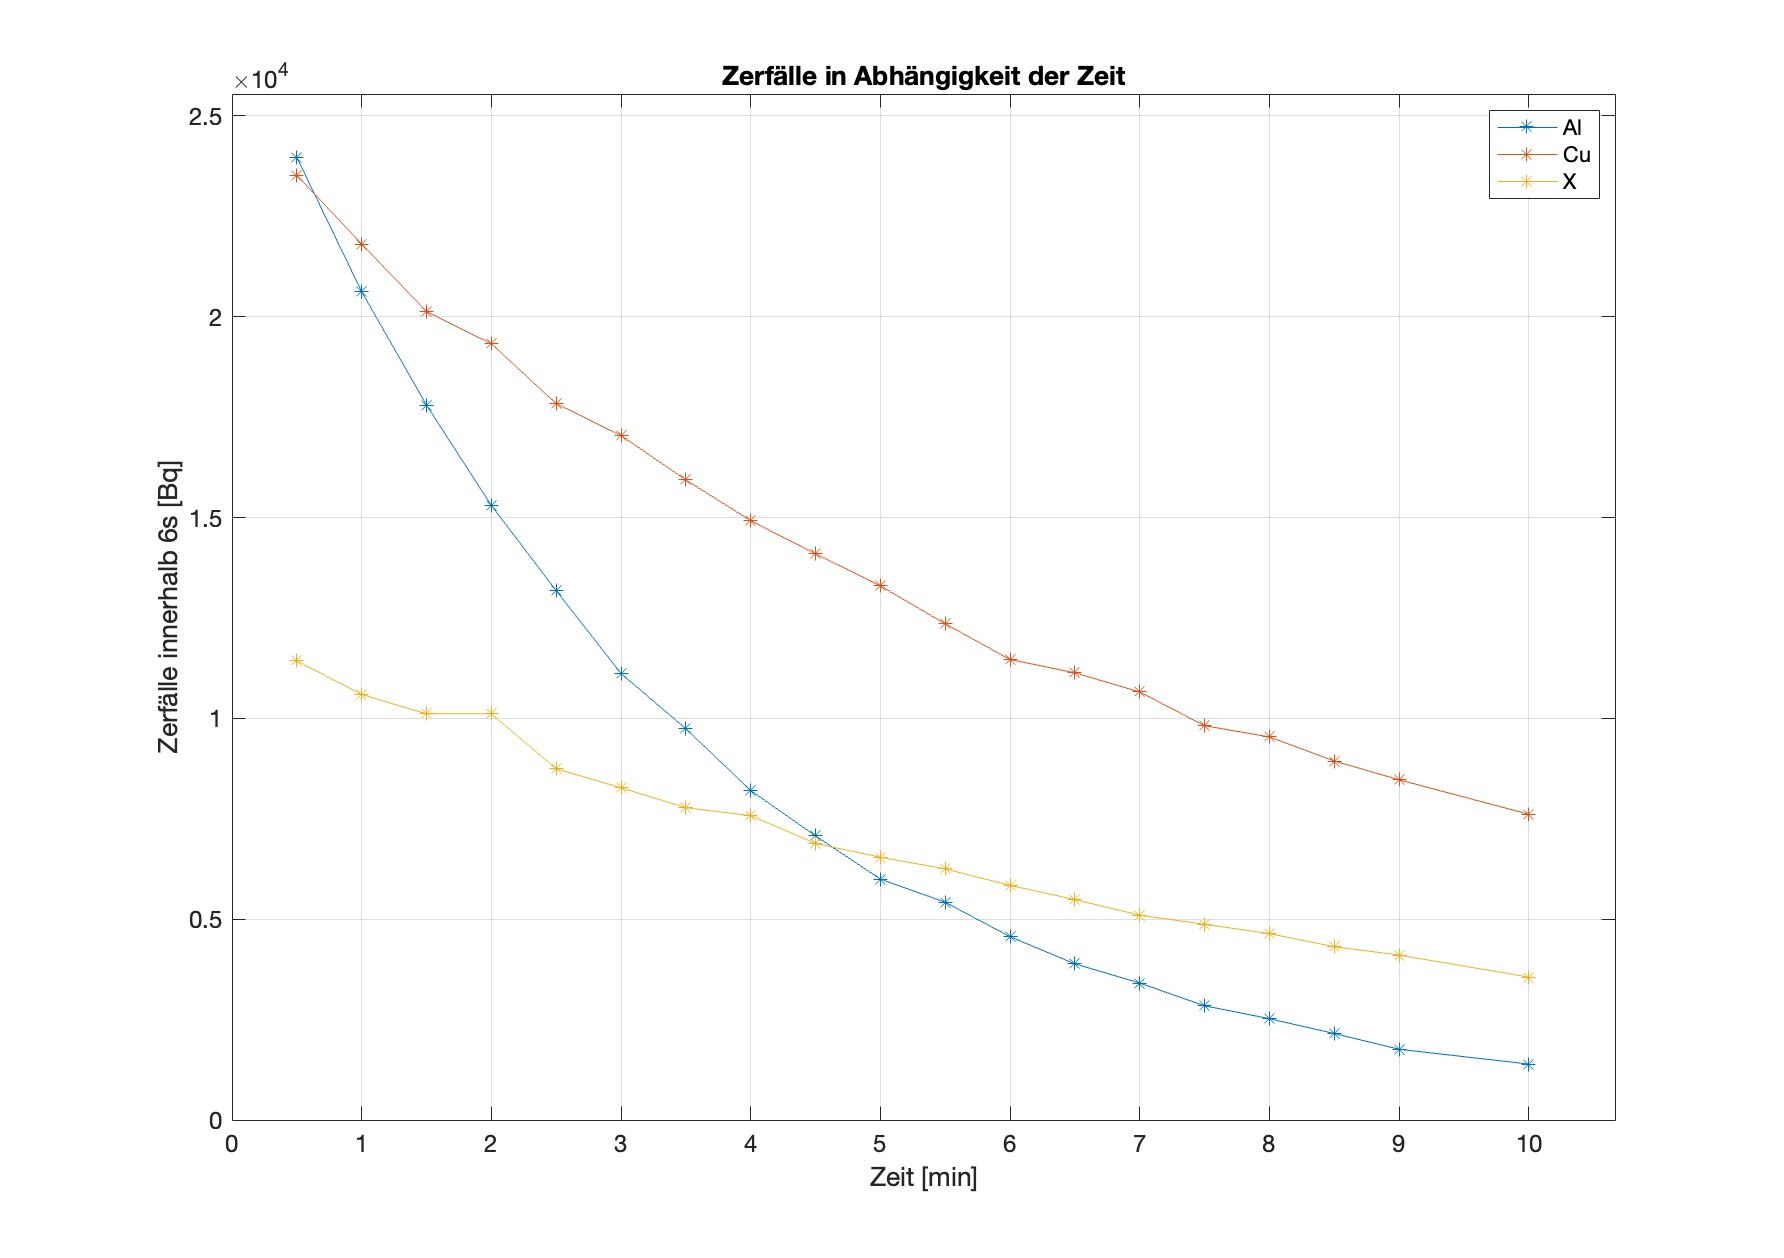
\includegraphics[width=\textwidth]{Diagramm.png}
        \caption{Messwerte mit linearer Achse}
    \end{figure}
    \begin{figure}[H]
        \centering
        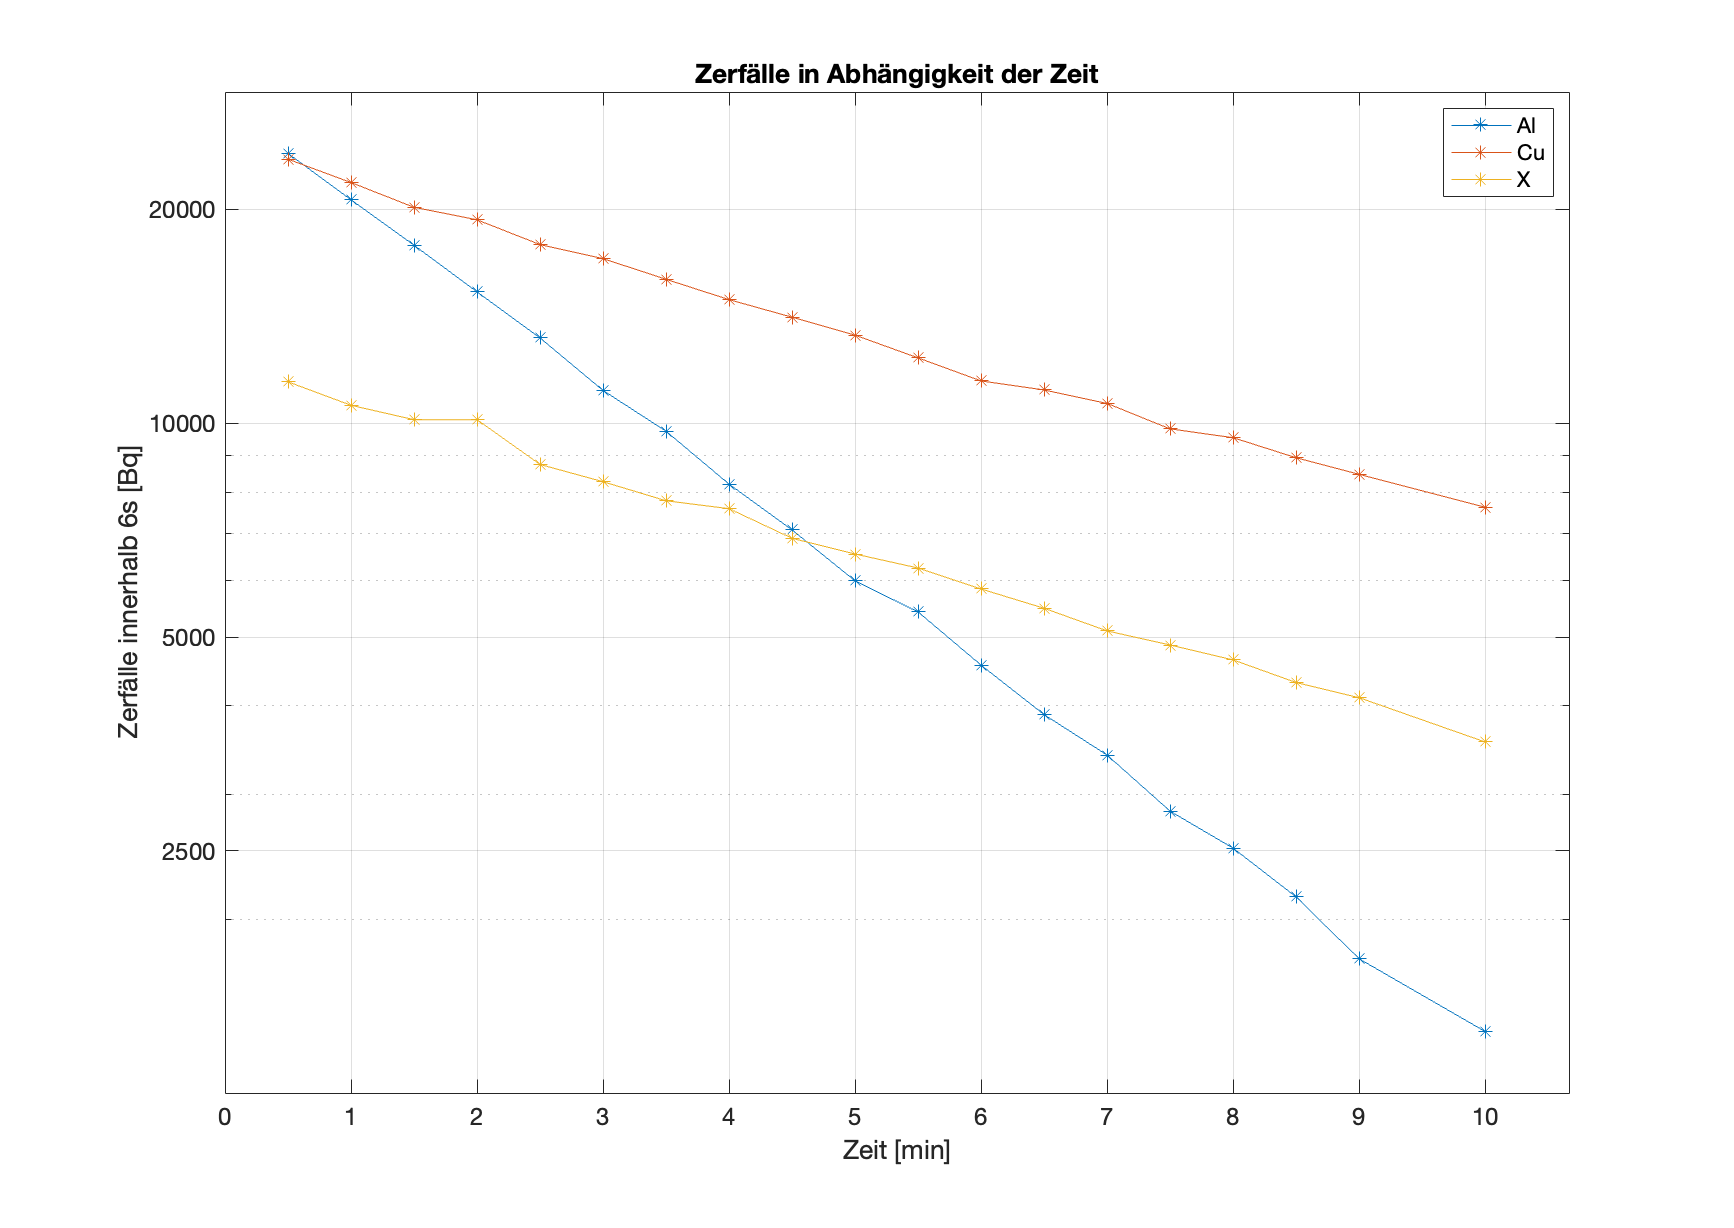
\includegraphics[width=\textwidth]{DiagrammLog.png}
        \caption{Messwerte mit logarithmischer Achse}
    \end{figure}

    \section{Bestimmung der Halbwertszeiten}
    \noindent
    Anhand der Abklingkurven kann man nun die Halbwertszeiten ablesen. \\
    Da der Verlauf der Aktivitätswerte durch den radioaktiven Zerfall einer Exponentialfunktion folgt, kann diese mittels exponentieller Regression näherungsweise bestimmt und anschließend die Halbwertszeit errechnet werden.
    Die aus den gemessenen Aktivitätswerten resultierenden Exponentialfunktionen sind folgende:
    \begin{align*}
        y_\text{Al} &= e^{10.2344\, -\, 0.3021 \cdot x} \\
        y_\text{Cu} &= e^{10.0940\, - \, 0.1182 \cdot x} \\
        y_\text{X} &= e^{9.3969\, -\, 0.1210 \cdot x}
    \end{align*}
    Nach der Bestimmung der Umkehrfunktionen lassen sich die Halbwertszeiten wie folgt berechnen:
    \begin{equation*}
        T_{1/2} = y^{-1}\left(\frac{y(100)}{2}\right) - 100
    \end{equation*}
    Die damit berechneten Halbwertszeiten lauten:
    \begin{align*}
        T_{1/2;\, \text{Al}}&: 2.29\, \text{min} \\
        T_{1/2;\, \text{Cu}}&: 5.86\, \text{min} \\
        T_{1/2;\, \text{X}}&: 5.72\, \text{min}
    \end{align*}
    Es handelt sich bei dem unbekannten Element also vermutlich um Messing.

    \section{Berechnen der Neutronenflussdichte am Bestrahlungsort}
    Es ergibt sich folgende Gleichung zu Berechnung der Neutronenflussdichte aus der Halbwertszeit von Kupfer:
    \begin{equation*}
        \Phi = \frac{\left(\text{Z}(t_b)\, -\, n_0\right) \cdot \text{AG}}{C \cdot m \cdot 0.309 \cdot N_L \cdot \sigma \cdot \left[1 - \exp(-\lambda \cdot t_b)\right]}
    \end{equation*}
    % @Artur: woher Aluminium?
    Es ergibt sich also für die Neutronenflussdichte ein Wert von $7,617 \cdot 10^{-19}\, \frac{n}{\text{cm}^2 \cdot \text{s}}$
\end{document}